\section{Output}
\subsection{Files}

Explain the created C++ files and executables, and how to use them.

\subsection{Two-scale algorithm}

Explain the structure of the two-scale algorithm classes and how they
work and are plugged together.

\begin{figure}[tb]
  \centering
  \tikzumlset{fill class=white}
  \begin{tikzpicture}
    \umlclass[x=0, y=0, type=abstract]{Beta\_function}{
      -- scale : double\\
      -- loops : unsigned\\
      -- numPars : unsigned
    }{
      + \umlvirt{display() : const Eigen::ArrayXd} \\
      + \umlvirt{set(v : const Eigen::ArrayXd\&) : void}\\
      + \umlvirt{beta() : Eigen::ArrayXd}\\
      + run\_to(scale : double, eps : double) : int\\
    }
    \umlclass[x=8, y=-12, template={T}]{MSSM}{}{}
    \umlclass[x=8, y=-8, type=abstract]{Two\_scale\_model}{}{
      + \umlvirt{calculate\_spectrum() : void}\\
      + \umlvirt{run\_to(scale : double, eps : double) : int}\\
      + \umlvirt{set\_precision(precision : double) : void}
    }
    \umlclass[x=0, y=-4]{MSSM\_susy\_parameters}{}{
      + display() : const Eigen::ArrayXd \\
      + set(v : const Eigen::ArrayXd\&) : void\\
      + beta() : Eigen::ArrayXd
    }
    \umlclass[x=0, y=-8]{MSSM\_soft\_parameters}{}{
      + display() : const Eigen::ArrayXd \\
      + set(v : const Eigen::ArrayXd\&) : void\\
      + beta() : Eigen::ArrayXd
    }
    \umlclass[x=0, y=-12]{MSSM$<$Two\_scale$>$}{}{
      + calculate\_spectrum() : void\\
      + run\_to(scale : double, eps : double) : int\\
      + set\_precision(precision : double) : void
    }
   \umlinherit{MSSM\_susy\_parameters}{Beta\_function}
   \umlinherit{MSSM\_soft\_parameters}{MSSM\_susy\_parameters}
   \umlinherit{MSSM$<$Two\_scale$>$}{MSSM\_soft\_parameters}
   \umlinherit{MSSM$<$Two\_scale$>$}{Two\_scale\_model}
   \umldep[arg1={$<<$bind$>>$}, mult1={T $\rightarrow$ Two\_scale}, pos1=0.5]{MSSM$<$Two\_scale$>$}{MSSM}
  \end{tikzpicture}
  \caption{Two-scale model class hierarchy}
  \label{fig:two-scale-model-class-hierarchy}
\end{figure}

\begin{figure}[tb]
  \centering
  \tikzumlset{fill class=white}
  \begin{tikzpicture}
    \umlclass[x=0, y=0, type=abstract]{Two\_scale\_model}{}{
      + \umlvirt{calculate\_spectrum() : void}\\
      + \umlvirt{run\_to(scale : double, eps : double) : int}\\
      + \umlvirt{set\_precision(precision : double) : void}
    }
    \umlclass[x=0, y=-4]{RGFlow$<$Two\_scale$>$}{}{
      + solve() : void
    }
    \umlclass[x=8, y=0]{Constraint$<$Two\_scale$>$}{}{
      + \umlvirt{apply() : void}\\
      + \umlvirt{get\_scale() : double}\\
      + \umlvirt{set\_model(model : Two\_scale\_model*) : void}
    }
    \umlclass[x=0, y=-7]{Initial\_guesser$<$Two\_scale$>$}{}{
      + \umlvirt{guess() : void}
    }
    \umlclass[x=0, y=-11, template={T}]{Initial\_guesser}{}{}
    \umlclass[x=8, y=-7]{Convergence\_tester$<$Two\_scale$>$}{}{
      + \umlvirt{accuracy\_goal\_reached() : bool}\\
      + \umlvirt{max\_iterations() : unsigned}
    }
    \umlclass[x=8, y=-11, template={T}]{Convergence\_tester}{}{}
    \umlclass[x=8, y=-4, template={T}]{RGFlow}{}{}
    \umldep[arg1={$<<$bind$>>$}, mult1={T $\rightarrow$ Two\_scale}, pos1=0.5]{RGFlow$<$Two\_scale$>$}{RGFlow}
    \umldep[mult1=1..*]{RGFlow$<$Two\_scale$>$}{Two\_scale\_model}
    \umldep[mult1=1..*]{RGFlow$<$Two\_scale$>$}{Constraint$<$Two\_scale$>$}
    \umldep{RGFlow$<$Two\_scale$>$}{Initial\_guesser$<$Two\_scale$>$}
    \umldep{RGFlow$<$Two\_scale$>$}{Convergence\_tester$<$Two\_scale$>$}
    \umldep[mult1={$<<$bind$>>$}, arg1={T $\rightarrow$ Two\_scale}, pos1=0.5]{Initial\_guesser$<$Two\_scale$>$}{Initial\_guesser}
    \umldep[mult1={$<<$bind$>>$}, arg1={T $\rightarrow$ Two\_scale}, pos1=0.5]{Convergence\_tester$<$Two\_scale$>$}{Convergence\_tester}
  \end{tikzpicture}
  \caption{Two-scale renormalization group solver class hierarchy}
  \label{fig:two-scale-rgflow-class-hierarchy}
\end{figure}

\subsection{Lattice algorithm}

Explain the structure of the lattice algorithm classes and how they
work.
